% 02.06.2016 12:00 CET last changed by a.holzinger
% General Template for LNCS and LNAI contributions based on llncs, adapted by ah
% Many thanks to the TRS team
% In case of using eps compile via 1) TeXify and then proceed with 2) dvi2pdf
%
\documentclass{llncs}
\usepackage{float}

\usepackage[dvips]{graphicx}
\usepackage[ruled,vlined]{algorithm2e}
\usepackage{amsfonts}
\usepackage{amssymb}
\usepackage{amsmath}
\usepackage{mathtools}

\providecommand{\abs}[1]{\lvert#1\rvert}
\providecommand{\norm}[1]{\lVert#1\rVert}

\usepackage{calc}
\usepackage{subfigure}

\usepackage{color}
\usepackage{soul}
\usepackage{comment}

\newtheorem{prop}{Property}

\newenvironment{Bitemize}{\renewcommand\labelitemi{\textbullet}\begin{itemize}}{\end{itemize}}

\begin{document}

\title{The more the merrier - Federated learning from graph based recommendations}

% \author{Bernd Malle\inst{1}\inst{2}, Peter Kieseberg\inst{1}\inst{2}, Edgar Weippl\inst{2}, Andreas Holzinger\inst{1}}

%\institute{Holzinger Group HCI-KDD \\
%Institute for Medical Informatics, Statistics \& Documentation\\
%            Medical University Graz, Austria\\
%            \texttt{b.malle@hci-kdd.org}
%\and
%SBA Research gGmbH, Favoritenstraße 16, 1040 Wien \\
%			\texttt{PKieseberg@sba-research.org}
%}
	
\maketitle

% ==================================
%				ABSTRACT
% ==================================
\begin{abstract}
	
With Google's \textit{Federated Learning} \& Facebook's introduction of client-side NLP into their chat service, the era of client-side Machine Learning has finally begun. While interesting ML approaches beyond the realm of toy examples were hitherto confined to large data-centers and powerful GPU's, exponential trends in computing technology and the introduction of billions of smartphones bring sophisticated processing pipelines within reach of even hand-held devices. Such approaches hold several promises: 1. Without the need for powerful server infrastructures, even small companies could be scalable to millions of users easily and cost-efficiently; 2. Since data only used in the learning process never need to leave the client, personal information can be used free of privacy and data security concerns; 3. Since privacy is preserved automatically, the full range of personal information on the client device can be utilized for learning; and 4. without round-trips to the server, results like recommendations can be made available to users much faster, resulting in enhanced user experience. In this paper we propose an architecture for federated learning from personalized, graph based recommendations computed on client devices, collectively creating \& enhancing a global knowledge graph. In this network, individual users will 'train' their local recommender engines, while a server-based voting mechanism aggregates the developing client-side models, preventing over-fitting on highly subjective data.

\medskip

\textbf{Keywords}: machine learning, federated learning, interactive learning, the local sphere, graph based recommendations, personalized ML models, distributed bagging


\end{abstract}

\renewcommand{\thesubfigure}{\thefigure.\arabic{subfigure}}
\makeatletter
\renewcommand{\p@subfigure}{}
\renewcommand{\@thesubfigure}{\thesubfigure:\hskip\subfiglabelskip}
\makeatother


% ==================================
%			INTRODCUTION
% ==================================
\section{Introduction and Motivation for Research}
\label{sect:intro_motivation}

\begin{figure}[H]
	\begin{center}
		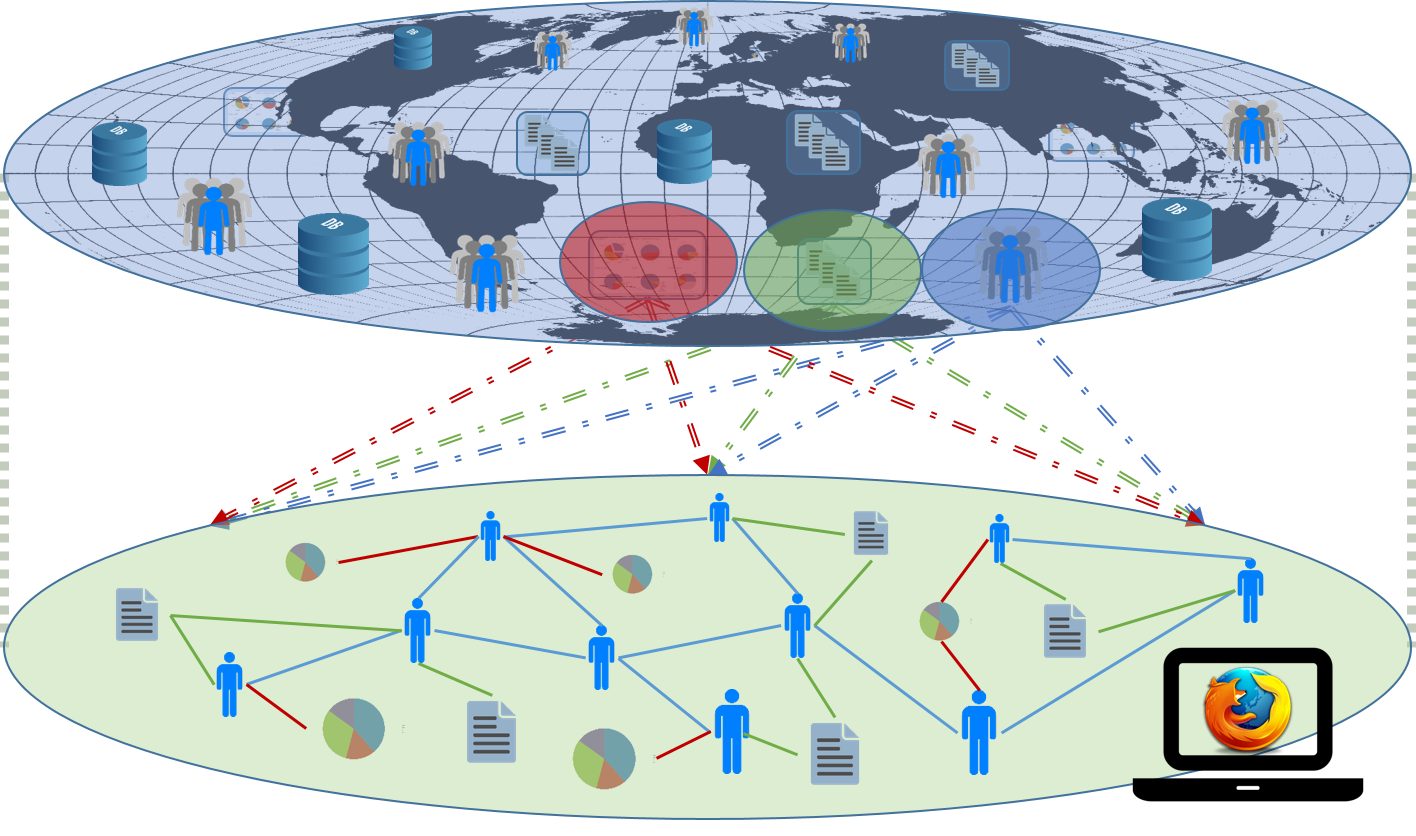
\includegraphics[width=0.9\textwidth]{figures/local_sphere}
		\caption{Publish-subscribe mechanism on a client constantly synchronizing a subsample of a \textit{global database} to constitute what we term the \textit{local sphere}}
		\label{fig:anon_categories}
	\end{center}
\end{figure}




\cite{leskovec2006recpatterns}
\cite{leskovec2006samplinggraphs}
\cite{leskovec2007blogpatterns}

\cite{mcmahan2016communication}
\cite{konevcny2016federatedlearning}
\cite{konevcny2016federatedoptimization}
\cite{2017secureaggregation}

\cite{shi2012climf}


\newpage

\bibliographystyle{plain}
\bibliography{references}

\end{document}


% \begin {comment}
% \section{Glossary and Key Terms}
% NOTE: this section may not to be used for a conference
% \textbf{Note: This is only for use when producing a Springer LNCS SOTA State-of-the-Art-Analysis paper}
% \\[0,2cm]
% \emph{SaNGreeA} is the abbreviation for Social Network Greedy Anonymization, which describes an anonymization algorithm which takes into account information loss as well as structural loss (from anonymizing the neighborhood of a network node). It is said to be greedy as it uses greedy clustering under the hood in order to avoid having to sift through an exponential solution space to find an optimum.
% \end{comment}
